\documentclass[10pt,landscape]{article}
\usepackage{multicol}
\usepackage{calc}
\usepackage{ifthen}
\usepackage[a4paper,landscape]{geometry}
\usepackage{hyperref}
\usepackage{tcolorbox}
\usepackage{graphicx}

\graphicspath{ {images/} }

% This sets page margins to .5 inch if using letter paper, and to 1cm
% if using A4 paper. (This probably isn't strictly necessary.)
% If using another size paper, use default 1cm margins.
\ifthenelse{\lengthtest { \paperwidth = 11in}}
	{ \geometry{top=.5in,left=.5in,right=.5in,bottom=.5in} }
	{\ifthenelse{ \lengthtest{ \paperwidth = 297mm}}
		{\geometry{top=1cm,left=1cm,right=1cm,bottom=1cm} }
		{\geometry{top=1cm,left=1cm,right=1cm,bottom=1cm} }
	}

% Turn off header and footer
\pagestyle{empty}


% Redefine section commands to use less space
\makeatletter
\renewcommand{\section}{\@startsection{section}{1}{0mm}%
                                {-1ex plus -.5ex minus -.2ex}%
                                {0.5ex plus .2ex}%x
                                {\normalfont\large\bfseries}}
\renewcommand{\subsection}{\@startsection{subsection}{2}{0mm}%
                                {-1explus -.5ex minus -.2ex}%
                                {0.5ex plus .2ex}%
                                {\normalfont\normalsize\bfseries}}
\renewcommand{\subsubsection}{\@startsection{subsubsection}{3}{0mm}%
                                {-1ex plus -.5ex minus -.2ex}%
                                {1ex plus .2ex}%
                                {\normalfont\small\bfseries}}
\makeatother

% Define BibTeX command
\def\BibTeX{{\rm B\kern-.05em{\sc i\kern-.025em b}\kern-.08em
    T\kern-.1667em\lower.7ex\hbox{E}\kern-.125emX}}

% Don't print section numbers
\setcounter{secnumdepth}{0}


\setlength{\parindent}{0pt}
\setlength{\parskip}{0pt plus 0.5ex}


% Colored boxes
% new tcolorbox environment
% #1: tcolorbox options
% #2: color
% #3: box title
\newtcolorbox{textbox}[3][]
{
  colframe = #2!25,
  colback  = #2!10,
  coltitle = #2!20!black,
  title    = #3,
  #1,
}


% -----------------------------------------------------------------------

\begin{document}

\raggedright
\footnotesize
\begin{multicols}{3}


% multicol parameters
% These lengths are set only within the two main columns
%\setlength{\columnseprule}{0.25pt}
\setlength{\premulticols}{1pt}
\setlength{\postmulticols}{1pt}
\setlength{\multicolsep}{1pt}
\setlength{\columnsep}{2pt}

\begin{center}
     \Large{CCNA Summary} \\
\end{center}

\section{CCNA Routing \& Switching \textit{200-120}}

\subsection{Understanding Networks and their Building Blocks}
\subsubsection{What is a network}
\paragraph{}
A network is nothing more than a collection of interconnected devices. A network is a tool to decrease cost, time,
and effort to increase productivity of people. For example by sharing files between offices a company can share data
between them is real-time. Networks reduces cost by sharing printers and other divices between multiple clients.
\paragraph{}
To connect to a network you'll need a \textbf{Network Interface Card (NIC)}, this connects to a network via a cable (e.g. Ethernet).
A NIC handles layer 1 and 2 (physical and network), the other layers are deligated to software layers in the layers above layer 2.

\subsubsection{Hubs and Switchers}
\paragraph{}
 To connect more than two devices with eachother you need to use a \textit{Hub} or a \textit{switch}.
\paragraph{}
A hub has two mayor disadvantages over a switch:
\begin{itemize}
	\item A hub repeats the information of one host to all other connected hosts. Even if the message is only meant for one
	other client.
	\item A hub can process only one message at a time. If multiple clients send a message at the same time a collision occurs.
	This collision is called a collision domain (all clients connected to one hub share the same collision domain)
\end{itemize}
\paragraph{}
Switches don't have a collision domain, which makes it a more efficient and faster device for routing messages on a network.
So you cloud say that a switch breaks up a collision domain.
\paragraph{}
Clients can communicate via three ways over the network.
\begin{itemize}
	\item \textbf{Unicast} A host sends a message to one other host on the network.
	\item \textbf{Broadcast} A host sends a message to all other hosts on the network.
	\item \textbf{Multicast} A hsot sends a message to a couple of hosts on the network.
\end{itemize}
\paragraph{}
All hosts connected to a network are in the same \textbf{broadcast domain}, which means that a broadcast message will get picked
up by all connected hosts in the broadcast domain. Really large networks can have problems with to many broadcasts. A \textbf{router}
breaks up broadcast domains. Routers seperate networks from eachother and do not allow broadcasts between those networks.
\paragraph{}
Besides breaking up broadcast networks routers have other essential functions for making multiple interconnected networks possible:
\begin{itemize}
	\item \textbf{Packet Switching} Just like a switch, routers switch packets between networks.
	\item \textbf{Connect Networks} Routers allow connecting networks with eachother.
	\item \textbf{Path Selection} Routers can learn about connected networks and pick the best path to send messages between networks.
	\item \textbf{Packet Filtering} Routers can drop packets based on rules set by a network administrator.
\end{itemize}

\subsubsection{Networking Types}
\paragraph{}
There are two important types of networks: \textbf{Local Area Network (LAN)} and \textbf{Wide Area Network (WAN)}. LANs are smaller
networks most of the time, you'll find them in your home, at work, and at school. They cover a small area like a floor or a building.
They can transfer a large amount of data. WANs cover areas like cities, countries, or continents, they connect LANs across areas
they cover.

\subsubsection{OSI Reference Model}
\paragraph{}
The OSI layer: \\
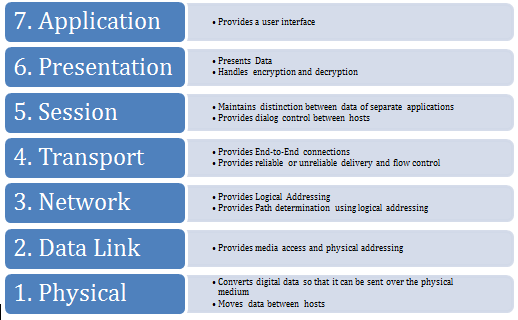
\includegraphics[width=7.5cm]{osi_layer}

Encapsulation of the different layers. Note that layer 2 encapsulate the layer packet on both sides. \\
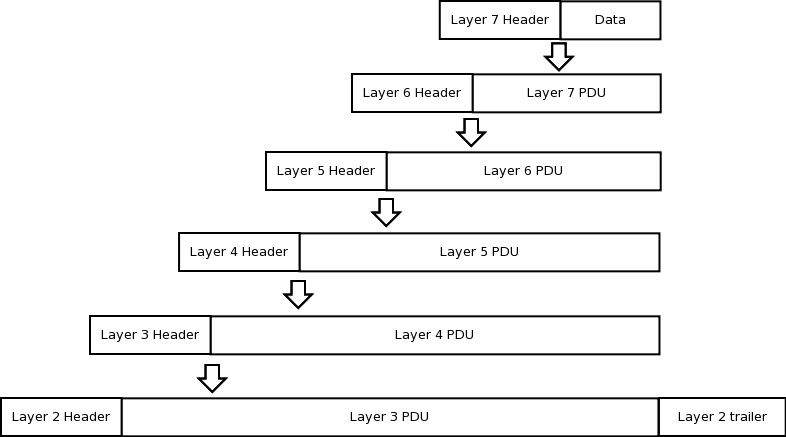
\includegraphics[width=7.5cm]{data_encapsulation}

\subsubsection{TCP/IP Model}
\paragraph{}
The TCP/IP Model is a stripped down version of the OSI Model. \\
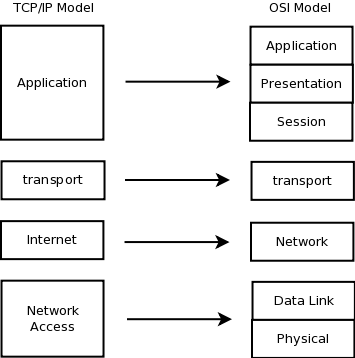
\includegraphics[width=5cm]{TCP_IP_model}

\subsubsection{Transport Control Protocol (TCP)}
\paragraph{}
TCP is a layer 3 protocol and is encapsulated by layer (Internet) and encapsulates the application layer. The protocol
uses a three-way handshake (SYN, SYN ACK, SYN ACK). After the handshake it breaks down the data of the application layer
into segments and ads its own header at the front of the fragement and sends it to layer 1 (Network Access).
\paragraph{}
The size of a TCP packet is based on the MTU (maximum transmission unit), a packet can never be bigger than the MTU
so most of the time the data of the application layer will be broken up into segments.
\paragraph{}
TCP also handles flow control, how fast a host can send data to the client. This is done based on a \textit{window}
this window scales up and down depending on the how full the window is. If a host doesn't get enough ACK responses
it will decrease the window size, it will increase the window size if it continiously receives ACK responses.
\paragraph{}
If the host doesn't get an ACK back it will resend the message that have not been ACKed. This can be done because
eacht TCP header contains a \textit{sequence number} so the host can see which packets have been ACKed. This sequence number
is also used too reorder the packages in the right order to sent it to the application layer.

\subsubsection{UDP}
\paragraph{}
UDP is like TCP a protocol on the Internet layer, that is the only thing they have in common. UDP doesn't have knowledge of
connections or does anything to make sure the package is send and received. The advantage of UDP over TCP is that is doesn't
have the overhead of TCP (retransmitting packages, keeping track of connections etc.).

\subsubsection{IP (IPv4 only)}
\paragraph{}
This is the backbone of the internet, it allows hosts to connect to eachother. Routers uses IP addresses to route IP packets from
network to network.

\subsection{IP Addressing and Subnets}
\begin{textbox}{gray}{TODO}
	This chapter is not yet complete!
\end{textbox}

\subsection{Introduction to Cisco Routers, Switches and IOS}
\begin{textbox}{gray}{TODO}
	This chapter is not yet complete!
\end{textbox}

\subsection{Introduction to IP Routing}
\begin{textbox}{gray}{TODO}
	This chapter is not yet complete!
\end{textbox}

\subsection{Routing Protocols}
\subsubsection{RIPv1 \& RIPv2}
\paragraph{}
RIP is a \textit{distance vector} protocol, the only widely used routing protocol that uses the distance vector protocol today.
\paragraph{}
RIPv1 was defined as a \textit{classful} protocol. Therefore it does not advertise subnet mask information and assumes the default subnest mask based on the class of the network.
\paragraph{}
When a router starts up, it will automatically add the connected networks to its routing table, denoting them with a \verb!C!.
If RIP is enabled, the router broadcasts its routing table. Neighbouring routers router with RIP enabled will receive the broadcast update and add the routes to their own routing tables.
Each RIP enabled router will broadcast its routing table this way, therefore the routing table will converge accross the network.
\paragraph{}
RIP has the following characteristics:
\begin{itemize}
	\item RIP sends out its \textit{entire} routing table every 30 seconds.
	\item Has a maximum hop count limit of 15.
	\item Implements split horizon, route poisoning and holddown timers to prevent routing loops.
	\item High convergence time.
\end{itemize}
\paragraph{}
RIP uses 4 different timers:
\begin{description}
	\item[Router update timer] Interval between the routing table broadcasts.
	\item[Router invalid timer] If a router does not head any updates about a route, it will consider that route as invalid.
	\item[Holddown timer] When a route becomes invalid, it enters into holddown state. The route will remain in the routing table but the router will not accept any updates regaring this rout unless the metric is equal to or better than the existing metric.
	\item[Router flush timer] While a route is in holddown state, the route is still in the routing table and will remain so for the duration specified by the flush timer.
\end{description}

\subsubsection{Enhanced Interior Gateway Routing Protocol (EIGRP)}
\paragraph{}
EIGRP is a Cisco Proprietary classless routing protocol. It takes various features of \textit{distance vecor} and \textit{link state} protocols to overcome the disadvantages of a distance vector protocol.
\paragraph{}
EIGRP uses the following features of a \textit{distance vector protocol}:
\begin{itemize}
	\item Hop count limit of 100 by default (\textit{up to 255}).
	\item Uses \textit{routing-by-rumor} mechanism.
	\item Implements loop avoidance techniques.
\end{itemize}
From a \textit{link state protocol} it inherits:
\begin{itemize}
	\item Neighbour discovery and periodically checking their state.
	\item Only sends updates when changes occur.
\end{itemize}
\begin{textbox}{gray}{TODO}
	This chapter is not yet complete!
\end{textbox}

\subsubsection{Open Shortest Path First (OSPF)}
\paragraph{}
OSPF is a \textit{link state protocol}. Besides it is also an open standard protocol, which allows OSPF to be used in a multivendor network.
Compared to EIGRP, OSPF is a more complex protocol. The features of OSPF are:
\begin{itemize}
	\item Works on the concept of Areas and Autonomous systems.
	\item Highly scalable.
	\item Support VLSM/CIDR and dis-contiguos networks.
	\item Does not have a hop count limit.
	\item Works in multivender environments.
	\item Minimizes updates betweens neighbors.
	\item And many more features...
\end{itemize}
\begin{textbox}{gray}{TODO}
	This chapter is not yet complete!
\end{textbox}

\subsection{Switching and Spanning Tree Protocol}
\begin{textbox}{gray}{TODO}
	This chapter is not yet complete!
\end{textbox}

\subsection{VLANs and VTP}
\subsection{MAC address table}
\paragraph{}
The ultimate goal of a switch it to carry frames from source to destination based on the MAC. Switch maintains a MAC Address Table. When a switch reveives a frame it does one of these 4 type of casts
\begin{description}
	\item[Known unicast] the switch has an entry in its MAC Address Table so it forwards the frame towards the associated interface
	\item[Unkown Unicast] the switch has no entry in its MAC Address Table and forwards a copy of the frame out of all interface, except the ingress port.
	\item[Broadcast] same as unknown unicast. There isn't much difference between Unknown Unicast en Broadcasting.
	\item[Multicast] the switch floods frame identically to unknown unicasts and broadcasts, unless certain multicast optimizations are configured.
\end{description}
\subsection{VLAN}
\paragraph{}
VLAN allows the network to be segmented based on factors like: function, location or department. VLAN creates a logical broadcast domain that can span multiple physical LAN segment.
Some of the benefits are:
\begin{itemize}
	\item Security
	\item Cost Reduction
	\item Better Performance
	\item Reduce size of broadcast domains
	\item Simple management
	\item Improved IT staff effiency
\end{itemize}
\paragraph{}
There are 5 types of VLAN:
\begin{description}
	\item[Data VLAN] Carries user-generated traffic. VLAN carrying voice or management traffic would not be a data VLAN (Data VLAN also called User VLAN)
	\item[Default VLAN] Default VLAN in Cisco switches is VLAN 1. And all switch ports become part of the default VLAN after initial boot up.
	\item[Native VLAN] A native VLAN is assigned to an 802.1Q trunk port. The 802.1Q trunk port places untagged traffic on the native VLAN, which by default is VLAN 1.
	\item[Management VLAN] A management VLAN is any VLAN configured to access the management capabilities of a switch. VLAN 1 is the management VLAN by default
	\item[Voice VLAN] A separate VLAN is needed to support Voice over IP (VoIP). Needs: Assured bandwidth, Transmission,
\end{description}
\paragraph{}
VLAN's wouldnt be useful without trunks. A VLAN trunk extends VLANs across an entire network. Cisco supports IEEE 802.1Q for coordinating trunks on Fast Ethernet, Gigabit Ethernet, and 10-Gigabit Ethernet interfaces. 
\textit{switchport access vlan 10 } assigns a VLAN to an interface port. 

\subsection{VLAN Routing}
\paragraph{}
Without a router VLAN cannot be routed through the network regardless of the device used, the process of forwarding network traffic from one VLAN to another VLAN using routing is known as inter-VLAN routing. There are three types. 
\begin{description}
	\item[Legacy Inter-VLAN routing] performed by using different physical router interfaces to different physical switch ports. Needs a cable for each VLAN. switch port must be in acces mode  
	\item[Router-on-a-stick] ‘Router-on-a-stick’ is a type of router configuration in which a single physical interface routes traffic between multiple VLANs on a network. Makes use of subinterfaces. switch interface must be in trunk mode.  
	\item[Layer 3 switching using SVIs] Is out of scope for CCNA 
\end{description}

\begin{textbox}{gray}{TODO}
	This chapter is not yet complete!
\end{textbox}

\subsection{Network Security}
\subsubsection{Security Introduction}
\paragraph{}
Internet and networks are becoming more complex and mission critical. Through the recent years there has been an intergration of network infrastructures.
As a matter of fact, no computer system in the world can be completely secure no matter how good the security measures are. Probably the only way to fully secure a computer is to isolate it completely, restricting all physical and virtual access to it. Such a system would not be connected to any network and would probably be stored in a secured vault somewhere with no physical access
\paragraph{}
Cisco IOS software running on Cisco routers has several built-in security tools that can be used as part of a good overall security strategy. Probably the most important security tool in Cisco IOS software are access control lists (ACL)
\begin{description}
	\item[C] Confidentiality - prevents acces to sensative information
	\item[I] Integritiy - prevents unauthorized modification of data
	\item[A] Availability  - prevents the loss of acces to information
\end{description}
\paragraph{}
In a medium to large enterprise, the typical secured network is built around a recipe of a perimeter router, a firewall device, and an internal router:
\begin{description}
	\item[Perimeter Router] is the border between enterprise resources and the public network (internet)
	\item[Firewall] Firewall allows sophisticated control of traffic flow.
	\item[Internal Router]  provides addtional security by providing a point for further traffic control
	\item[DMZ] provides a buffer zone that seperates a trusted network from the untrusted network.
\end{description}
\paragraph{}
Vulnerabilities, Threats and Exploits:
\begin{description}
	\item[Vulnerability] - a weakness in a system or design which can be exploited by a threat
	\item[Threat] - threat is an external danger to the system have a vulnerability
	\item[Exploit] said to exist when computer code is actually developed to take advtanges of a vulnerability.
\end{description}

\subsubsection{Type of Attacks}
\paragraph{}
There are three major types of networks attacks:
\begin{itemize}
	\item  Reconnaissance Attacks
	\item  Access Attacks
	\item  Denial of Service
\end{itemize}
\subsubsection{Counter measures}
\paragraph{}
Physicial and Administrative security measures
\begin{itemize}
	\item Locks
	\item Biometric acces systems
	\item Security Traps
	\item IDS
	\item Safes
	\item Racks
	\item UPS
	\item Positive air-flow systems
	\item Fire Suppresion systems
\end{itemize}
\subsubsection{Port Security}
\paragraph{}
You can use port security feature to \textit{restrict} who can acces the network by connecting to a switchport.
\paragraph{}
You can specify which MAC addresses are allowed to acces the port. f a port is configured as a secure port and the maximum number of MAC addresses is reached, any additional attempts to connect by unknown MAC addresses will generate a security violation

There are three Secure MAC Address Types
\begin{description}
	\item[Static Secure ] manually configured MAC addresses. Are stored in address table and added to the running-config
	\item[Dynamic Secure] are dynmaically learned. Are stored in address table and are removed when the switch restarts
	\item[Sticky Secure] can either be manually or dynamically learned. stored in the address table and added to running-config Sticky Learning must be enabled by the command \textit{switchport port-security mac-address sticky}
\end{description}

\subsection{Access Lists}
\begin{textbox}{gray}{TODO}
	This chapter is not yet complete!
\end{textbox}

\subsection{Network Address Translation (NAT)}
\begin{textbox}{gray}{TODO}
	This chapter is not yet complete!
\end{textbox}

\subsection{Wide Area Networks}
\begin{textbox}{gray}{TODO}
	This chapter is not yet complete!
\end{textbox}

\subsection{Virtual Private Networks}
\begin{textbox}{gray}{TODO}
	This chapter is not yet complete!
\end{textbox}

\subsection{IPv6}
\subsubsection{IPv6 Introduction}
\paragraph{}
Due to the shortcomings of IPv4, the Internet Protocol version 6 (IPv6) has been created.
The main reason for migratig TCP/IP networks from IPv4 to IPv6 is the avaiable address space.
While IPv4 uses a 32-bit address, IPv6 uses a 128-bit address.
The change from IPv4 to IPv6 also impacts other protocols as well (\textit{OSPFv3, EIGRPv6, etc.}).
\paragraph{}
Just like IPv4, the main objective of IPv6 is to enable devices to forward packets through multiple routers so they arrive at the correct destination.
However, IPv6 contains a number of differences over IPv4:
\begin{itemize}
	\item Larger address space;
	\item Auto-configuration;
	\item The IPv6 header is \textit{not} similar to the IPv4 header;
	\item Extension headers/options;
	\item Authentication and privacy;
	\item Flow labels (\textit{QoS}).
\end{itemize}
\paragraph{}
There are thee types of IPv6 addresses:
\begin{description}
	\item[Unicast] Unique address for each interface.
	\item[Anycast] Multiple interfaces, packets are send to one (\textit{nearest}).
	\item[Multicast] Multiple interfaces, packets are send to all.
\end{description}
\begin{textbox}{green}{Key Concept}
	IPv6 broadcast addresses are special case of multicast addresses.
\end{textbox}
\paragraph{}
An IPv6 address is a 128-bit value, displayed as 8 groups of 4 hexadecimal digits.
For example: \verb!2001:0DB8:0000:0000:0006:0600:300D:527B!.
Leading zeros can be left out: \verb!2001:DB8:0:0:6:600:300D:527B!, one or more adjecent groups
of 16 bit of zeros can be replaced with the \verb!::! symbol (\textit{once!}): \verb!2001:DB8::6:600:300D:527B!.
\paragraph{}
IPv6 provides tow similar options for unicast addressing:
\begin{description}
	\item[Global Unicast] Similar to public IPv4 addresses. These addresses are allocated by the IANA. Each company is assigned a unique IPv6 address block called a \textit{global routing prefix}. Global Unicast addresses make up the majority of IPv6 addresses.
	\item[Unique Local] Similar to private IPv4 addresses. Can by used by when behind a IPv6 NAT and in networks that aren't connected to the internet.
\end{description}
\paragraph{}
IPv6 addresses can be identified by the initial bits of the address:
\begin{tabular}{@{}l@{}l@{}l@{}}
\textit{Address Type} & \textit{Binary Prefix} & \textit{IPv6 Notation} \\
Unspecified                       & %
        \verb!000…0 (128 bits)!   & %
        \verb!::/128!             \\
Loopback                          & %
        \verb!000…1 (128 bits)!   & %
        \verb!::1/128!            \\
Multicast                         & %
        \verb!1111 1111!          & %
        \verb!FF00::/8!           \\
Link-Local Unicast                & %
        \verb!1111 1110 10!       & %
        \verb!FF80::/10!          \\
Global Unicast                    & %
        \textit{everthing else}   & %
        \textit{everthing else}
\end{tabular}

\subsubsection{IPv6 Address Configuration}
\begin{textbox}{gray}{TODO}
	This chapter is not yet complete!
\end{textbox}
\subsubsection{OSPF version 3}
\begin{textbox}{gray}{TODO}
	This chapter is not yet complete!
\end{textbox}
\subsubsection{EIGRP for IPv6}
\begin{textbox}{gray}{TODO}
	This chapter is not yet complete!
\end{textbox}

\subsection{IP Services}
\begin{textbox}{gray}{TODO}
	This chapter is not yet complete!
\end{textbox}

\rule{0.3\linewidth}{0.25pt}
\scriptsize

\href{https://github.com/roaldnefs/ccna}{https://github.com/roaldnefs/ccna}

\end{multicols}
\end{document}
